% mnras_template.tex 
%
% LaTeX template for creating an MNRAS paper
%
% v3.0 released 14 May 2015
% (version numbers match those of mnras.cls)
%
% Copyright (C) Royal Astronomical Society 2015
% Authors:
% Keith T. Smith (Royal Astronomical Society)

% Change log
%
% v3.0 May 2015
%    Renamed to match the new package name
%    Version number matches mnras.cls
%    A few minor tweaks to wording
% v1.0 September 2013
%    Beta testing only - never publicly released
%    First version: a simple (ish) template for creating an MNRAS paper

%%%%%%%%%%%%%%%%%%%%%%%%%%%%%%%%%%%%%%%%%%%%%%%%%%
% Basic setup. Most papers should leave these options alone.
\documentclass[fleqn,usenatbib]{mnras}

% MNRAS is set in Times font. If you don't have this installed (most LaTeX
% installations will be fine) or prefer the old Computer Modern fonts, comment
% out the following line
\usepackage{newtxtext,newtxmath}
% Depending on your LaTeX fonts installation, you might get better results with one of these:
%\usepackage{mathptmx}
%\usepackage{txfonts}

% Use vector fonts, so it zooms properly in on-screen viewing software
% Don't change these lines unless you know what you are doing
\usepackage[T1]{fontenc}

% Allow "Thomas van Noord" and "Simon de Laguarde" and alike to be sorted by "N" and "L" etc. in the bibliography.
% Write the name in the bibliography as "\VAN{Noord}{Van}{van} Noord, Thomas"
\DeclareRobustCommand{\VAN}[3]{#2}
\let\VANthebibliography\thebibliography
\def\thebibliography{\DeclareRobustCommand{\VAN}[3]{##3}\VANthebibliography}


%%%%% AUTHORS - PLACE YOUR OWN PACKAGES HERE %%%%%

% Only include extra packages if you really need them. Common packages are:
\usepackage{graphicx}	% Including figure files
\usepackage{amsmath}	% Advanced maths commands


%%%%%%%%%%%%%%%%%%%%%%%%%%%%%%%%%%%%%%%%%%%%%%%%%%

%%%%% AUTHORS - PLACE YOUR OWN COMMANDS HERE %%%%%

% Please keep new commands to a minimum, and use \newcommand not \def to avoid
% overwriting existing commands. Example:
%\newcommand{\pcm}{\,cm$^{-2}$}	% per cm-squared

%%%%%%%%%%%%%%%%%%%%%%%%%%%%%%%%%%%%%%%%%%%%%%%%%%

%%%%%%%%%%%%%%%%%%% TITLE PAGE %%%%%%%%%%%%%%%%%%%

% Title of the paper, and the short title which is used in the headers.
% Keep the title short and informative.
\title[Short title, max. 45 characters]{Population III Sink Particle mergers and IMF convergence: Resolution Study}

% The list of authors, and the short list which is used in the headers.
% If you need two or more lines of authors, add an extra line using \newauthor
\author[L. R. Prole]{
Lewis R Prole,$^{1}$\thanks{E-mail: Prolel@cardiff.ac.uk}
$.$
$$
$$
\\
% List of institutions
$^{1}$Cardiff University School of Physics and Astronomy\\
$$
$$
}

% These dates will be filled out by the publisher
\date{Accepted XXX. Received YYY; in original form ZZZ}

% Enter the current year, for the copyright statements etc.
\pubyear{2020}

% Don't change these lines
\begin{document}
\label{firstpage}
\pagerange{\pageref{firstpage}--\pageref{lastpage}}
\maketitle

% Abstract of the paper
\begin{abstract}
The Population III initial mass function (IMF) is currently unknown, but recent studies agree that fragmentation of primordial gas gives a broader IMF than the initially accepted singular star per halo. Sink particles introduced at high densities can prevent artificial fragmentation of the gas once the mesh stops refining, but an incorrect choice of sink particle creation density will effect the resulting IMF. We present the evolution of the  total number of sinks formed and the total mass of the combined sinks, for five different sink creation densities, and the difference in velocity power spectra just before sink creation. This study also introduces sink mergers into AREPO.
\end{abstract}

% Select between one and six entries from the list of approved keywords.
% Don't make up new ones.
\begin{keywords}
keyword1 -- keyword2 -- keyword3
\end{keywords}

%%%%%%%%%%%%%%%%%%%%%%%%%%%%%%%%%%%%%%%%%%%%%%%%%%

%%%%%%%%%%%%%%%%% BODY OF PAPER %%%%%%%%%%%%%%%%%%

\section{Introduction}
The first stars, known as Population III (Pop III) stars, are responsible for the first ionising radiation which began the epoch of re-ionisation, and when they died as supernovae, they injected the interstellar medium (ISM) with the first metals, which would go on to form the next generation (Pop II) of stars. During their formation, the primordial magnetic seed field was amplified via the small-scale magnetic dynamo (REF), which may have been the first step in converting the small scale chaotic fields into the coherent, large scale galactic magnetic fields observed today. Evidently the initial mass function (IMF) of Pop III stars has a huge effect on the evolution of the Universe. Initially it was thought that Pop III stars formed in isolation, and were massive (REF), yet further studies showed they were susceptible to fragmentation in the presence of subsonic turbulence (REF). Since then, numerical studies have attempted to improve the picture of Pop III star formation by including feedback mechanisms (REF), live dark matter (DM) potentials (REF) and magnetic fields (REF). Despite this, the Pop III IMF is still in dispute, and there are still many factors left to study.

The Jeans length $\lambda_J$ of a structure of given density and temperature marks the maximum size it can achieve before thermal pressure cannot resist against gravitational collapse. Hence artificial fragmentation occurs in hydrodynamic codes if the local $\lambda_J$ falls below the size of mesh cells $\Delta x$. To prevent this, the mesh refines itself based on the local $\lambda_J$, which depends on the temperature and density of the gas. The Truelove condition (REF) requires a Jeans number $\Delta x/\lambda_J$ of 0.25, corresponding to at least 4 cells spanning across any $\lambda_J$ to prevent artificial fragmentation. Numerical simulations cannot refine indefinitely as the gas gets denser, and at higher densities (smaller $\lambda_J$), it becomes computationally expensive to refine further. Sink particles (REF: Bate 1995) provide an alternative to indefinite refinement, they are non-gaseous particles that contain all of the mass within the area they occupy and can accrete matter from their surrounding cells. As they cannot fragment, either naturally or artificially, their implementation at high densities  overcomes the Jeans refinement criteria. In present day star formation simulations, the sink creation density is chosen to be $\sim 10^{10}gcm^{-3}$ (e.g. REF), corresponding to the first adiabatic core (REF). During an adiabatic collapse , the radial density profile is flat within the central $\lambda_J$ (REF: Larson69), so the radius of the of sink particle is chosen to be the Jeans length at the creation density and temperature. In primordial star formation, there is no clear 'first core' (REF Omiki graph), and so the appropriate time to introduce a sink particle is unclear. Sink particles are not a perfect solution to the indefinite refinement problem, and authors choice of sink particle creation density will change the morphology  of the resulting cluster. This paper explores the effect of varying the sink particle creation density within the frame of primordial Pop III gas collapse. The most important parameters to track are the total number of sinks formed and the total combined mass of the sinks.

\section{Sink particles}

The radius of a sink particle is chosen to be $\lambda_J$ corresponding to the sink creation density, given by


\begin{equation}
    \lambda_J=\sqrt{  \frac{k_B T} {G \rho_{sink} (\mu m_p)}}.
	\label{eq:jeans}
\end{equation}

where $k_B$ is the Boltzmann constant, T is the temperature, $\rho_sink$ is the sink creation density, $\mu$ is the mean molecular weight and $m_p$ is the mass of a proton. To estimate $\lambda_J$ before running the simulation, an estimate of T at $\rho_{sink}$ is needed. To achieve this, a lower resolution simulation was performed without turbulence, resulting in 1 central star. The simulation was run up until the maximum creation density testing in this study was reached, figure REF shows the resulting relationship between density and temperature. This gives an effective relationship between $\rho$ and $\lambda_J$ using equation \ref{eq:jeans}. The sink radius was chosen to be 8 times smaller than $\lambda_J$ in compliance with the Truelove condition. This radius sets the minimum cell size and gravitational softening length of the simulation. The $\rho_{sink}$, T, $\lambda_J$, minimum cell volume and minimum gravitational softening lengths are given in table \ref{table:1}.

\begin{table}
	\centering
	\caption{Sink creation density, temperature, sink radius, minimum cell size and minimum gravitational softening lengths used in the study.}
	\label{table:1}
	\begin{tabular}{lcccr} % four columns, alignment for each
		\hline
		$\rho_{sink}$ [$gcm^{-3}$] & T [K] & $\lambda_J$ [cm] & $V_{min}$ [cm$^{3}$] & $L_{soft}$ [cm]\\
		\hline
		$10^{-10}$ & 2 & 1.37e14 & 5.10e39 & 1.72e13\\
		$10^{-9}$ & 4 & 4.56e13 & 1.86e38 & 5.70e12\\
		$10^{-8}$ & 5 & 1.53e13 & 6.95e36 & 1.91e12\\
		$10^{-7}$ & e & e & e & e\\
		$10^{-6}$ & e & e & e & e\\
		\hline
	\end{tabular}
\end{table}

\subsection{Sink mergers}
The total number of sinks formed is not representative of the IMF if they were allowed to bunch up and lie on top of one another. Similarity to REF(federath2010), we allow sinks to merge if they fit four criteria: they lie within eachothers accretion radius, they are moving towards eachother $(\nabla \cdot v) < 0$, their accelerations give $(\nabla \cdot a) <0$ and they are gravitationally bound. Since sink particles carry no thermal data, the last criteria simply requires that their gravitational potential well exceeds the kinetic energy of the system. When the criteria is met, the larger of the sinks gains the mass and linear momentum of smaller sink, and its position is shifted to the center of mass of the system. We allow multiple mergers per time-step based on mass hierarchy; if sink A is flagged to swallow sink B, and sink B is flagged to swallow sink C, then both B and C will be merged into sink A simultaneously. 

\section{Simulations}
Four iterations were performed with identical initial conditions with the moving mesh code AREPO (REF), varying the sink parameters as given in table \ref{table:1}. The chemistry used was the same as (REF clark), with abundances of H$_2$, H$^{+}$, D$^{+}$ and HD as x$_{\text{H}_{2}}$=10$^{-3}$, x$_{\text{H}^{+}}$=10$^{-7}$, $x_{\text{D}^{+}}$=2.6$\times$10$^{-12}$ and $x_{\text{HD}}$=3$\times$10$^{-7}$. The initial conditions consist of a Bonner Ebert sphere categorised by central density $n_c$=2$\times$10$^{-20}$ and radius R$_{\text{BE}}$=1.87pc, which was placed in a box of side length 4R$_{\text{BE}}$. The density was enhanced by a factor of 1.87 to promote collapse. A random velocity field was generated from the turbulent power spectrum $\propto k^{-2}$. The rms velocity was scaled to give a ratio of kinetic to gravitation energy $\alpha$=0.05 and the initial box temperature was 200K.

% Example figure
\begin{figure}
	% To include a figure from a file named example.*
	% Allowable file formats are eps or ps if compiling using latex
	% or pdf, png, jpg if compiling using pdflatex
	\hbox{\hspace{-0.8cm} 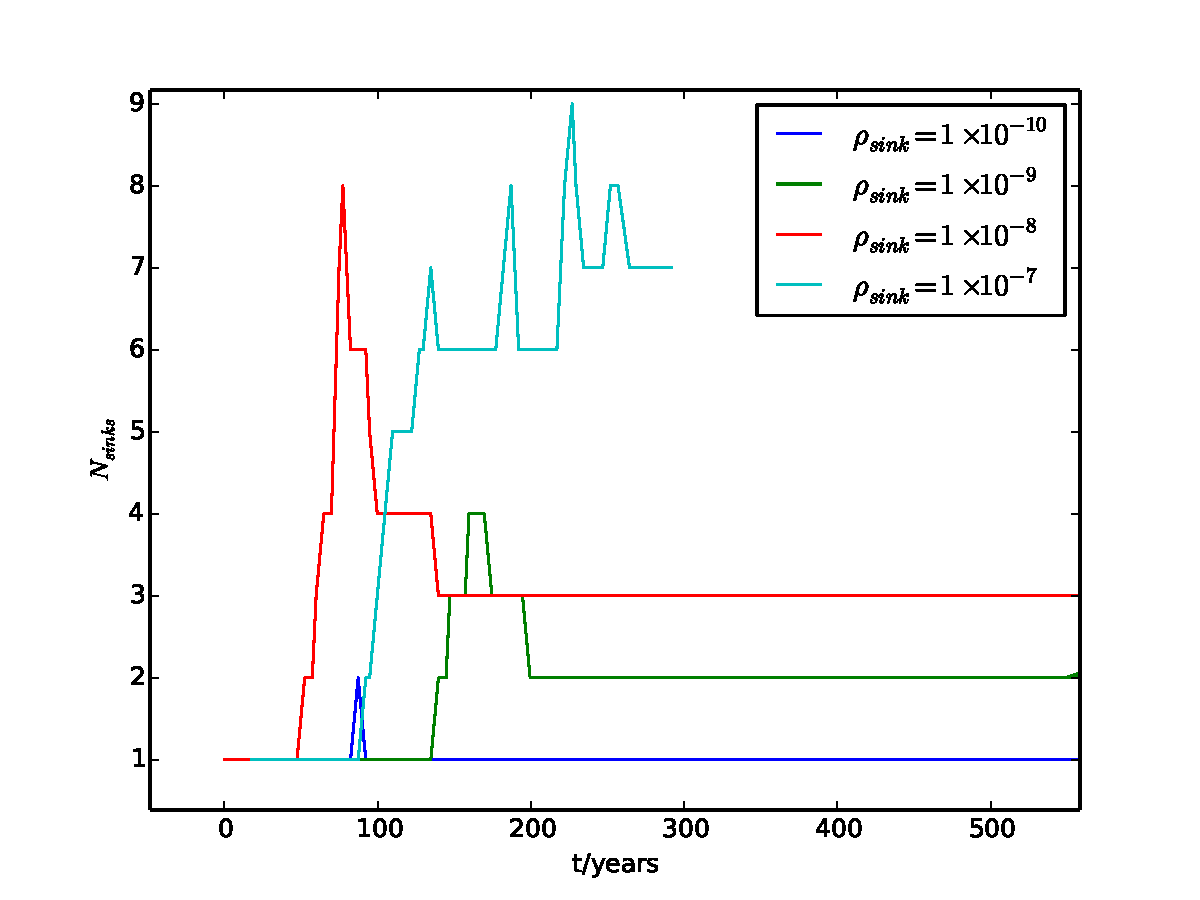
\includegraphics[scale=0.5]{sink_mergers_zoom.pdf}}
    \caption{Evolution of the number of sinks and the total mass of all sinks with sink mergers allowed.}
    \label{fig:example_figure}
\end{figure}

% Example table



\section{Conclusions}

The last numbered section should briefly summarise what has been done, and describe
the final conclusions which the authors draw from their work.

\section*{Acknowledgements}

The Acknowledgements section is not numbered. Here you can thank helpful
colleagues, acknowledge funding agencies, telescopes and facilities used etc.
Try to keep it short.

%%%%%%%%%%%%%%%%%%%%%%%%%%%%%%%%%%%%%%%%%%%%%%%%%%
\section*{Data Availability}

 
The inclusion of a Data Availability Statement is a requirement for articles published in MNRAS. Data Availability Statements provide a standardised format for readers to understand the availability of data underlying the research results described in the article. The statement may refer to original data generated in the course of the study or to third-party data analysed in the article. The statement should describe and provide means of access, where possible, by linking to the data or providing the required accession numbers for the relevant databases or DOIs.




%%%%%%%%%%%%%%%%%%%% REFERENCES %%%%%%%%%%%%%%%%%%

% The best way to enter references is to use BibTeX:

\bibliographystyle{mnras}
\bibliography{references.bib} % if your bibtex file is called example.bib



%%%%%%%%%%%%%%%%%%%%%%%%%%%%%%%%%%%%%%%%%%%%%%%%%%

%%%%%%%%%%%%%%%%% APPENDICES %%%%%%%%%%%%%%%%%%%%%

\appendix

\section{Some extra material}

If you want to present additional material which would interrupt the flow of the main paper,
it can be placed in an Appendix which appears after the list of references.

%%%%%%%%%%%%%%%%%%%%%%%%%%%%%%%%%%%%%%%%%%%%%%%%%%


% Don't change these lines
\bsp	% typesetting comment
\label{lastpage}
\end{document}

% End of mnras_template.tex